\section{Literature Review}
\begin{frame}[allowframebreaks]{Literature Review}

\textcolor{blue}{\textbf{Token-based/Lexing methods}}
\begin{figure}[h]
    \centering
    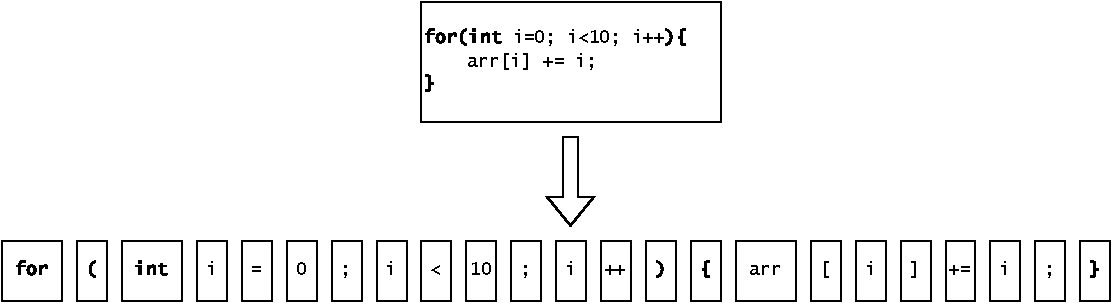
\includegraphics[width=0.8\linewidth]{images/lex.pdf}
    \caption{An example illustrating the lexing process \cite{hareretal2018}}
    \label{fig:token-based}
\end{figure}
\framebreak

\textcolor{blue}{\textbf{Token-based/Lexing methods}}
\medskip
\begin{itemize}
    \item These methods (\textit{e.g.} \cite{hareretal2018,cambronero2019deep,suman2020source}) use traditional vectorization techniques used in plain text (\textit{e.g.} Tf-Idf, word2vec), or use lexical analysis tools, to generate tokens.
    \item The tokens are then fed to a model in a similar fashion to plain text classifiers.
\end{itemize}
\medskip
\textbf{Problem with this approach:}
\begin{itemize}
    \item Treating source code as natural language texts can miss semantic information of source code \cite{zhang2019novel}.
\end{itemize}
\framebreak

\textcolor{blue}{\textbf{Abstract Syntax Tree (AST)-based Methods}}
\medskip
\begin{itemize}
    \item These methods use a language-specific parser to extract syntactic paths from source code.
    \item Each of the path and leaf-values of a path-context is mapped to its corresponding real-valued vector representation, or its embedding.
\end{itemize}
\medskip
\par There have been two methodologies proposed for AST-based techniques.
\framebreak

\textcolor{blue}{\textbf{Entire AST}}
\begin{figure}
\begin{center}
\begin{minipage}{0.3\textwidth}
    \centering
    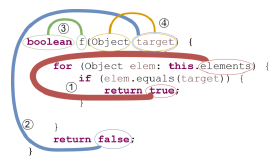
\includegraphics[width=\linewidth]{images/java.png}
    (a)
\end{minipage}%
\begin{minipage}{0.6\textwidth}
    \centering
    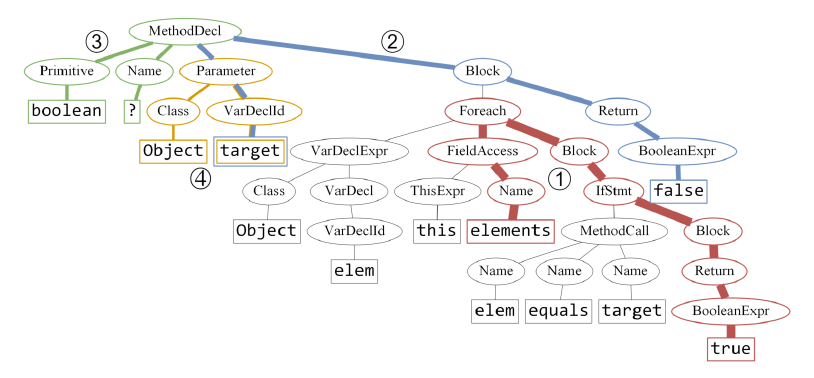
\includegraphics[width=\linewidth]{images/ast.png}
    (b)
\end{minipage}
\caption{(a) A Java method \cite{alon2019code2vec}, (b) Its AST \cite{alon2019code2vec}}
\label{fig:entire-ast}
\end{center}
\end{figure}
\framebreak

\textcolor{blue}{\textbf{Entire AST}}
\medskip
\par Given an AST,
\begin{itemize}
    \item This method (\cite{alon2019code2vec,compton2020embedding,azcona2019user2code2vec}) works on the entire tree,
    \item Selects paths from root to leaves on-by-one,
    \item Assigns a path-context
\end{itemize}
\medskip
\par\textbf{Problem with this approach:}
\begin{itemize}
    \item AST sizes are usually large, so computation complexity is a serious issue.
    \item Existing models have long term dependency problem \cite{zhang2019novel}.
\end{itemize}
\framebreak

\textcolor{blue}{\textbf{Splitting AST}}
\begin{figure}
    \centering
    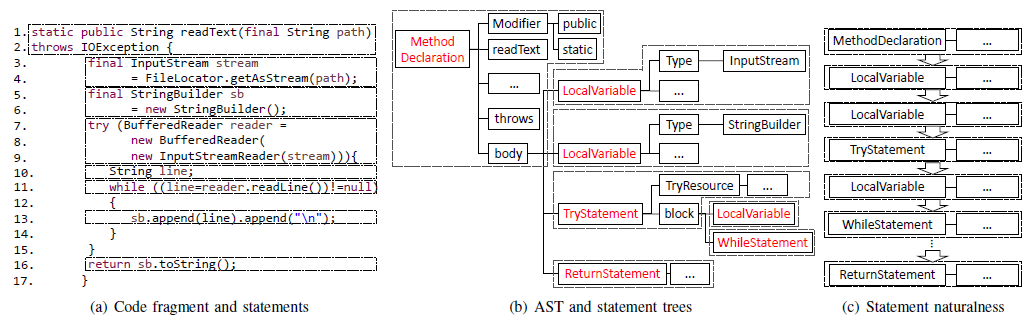
\includegraphics[width=0.9\linewidth]{images/split-ast.png}
    \caption{An example of AST statement nodes \cite{zhang2019novel}}
\end{figure}
\framebreak

\textcolor{blue}{\textbf{Splitting AST}}
\medskip
\begin{itemize}
    \item In this method \cite{zhang2019novel}, a neural network splits the large AST of one code fragment into a set of small trees at the statement level.
    \item Performs tree-based neural embedding on all statement trees.
    \item It produces statement vectors, which can represent the lexical and statement-level syntactical knowledge.
\end{itemize}
\medskip
\par\textbf{Problem with this approach \cite{zhang2019novel}:}
\begin{itemize}
    \item A definite efficiency is unknown.
    \item There is no improvement in performance.
\end{itemize}
\end{frame}